\section{绝对连续与相互奇异}
\label{sec:dens-ac-singular}

同一个可测空间上可以放很多测度：长度、点质量、计数测度以及它们的加权和。比较两个测度时，最粗也最基本的信息是它们怎样对待“可以忽略的集合”。本节固定可测空间$(X,\mathcal A)$上的两个非负测度，一个作为参考，一个作为要描述的目标，只用集合上的测度值回答两个问题：参考测度忽略的集合，目标测度是否也忽略；两个测度的质量能否分别集中在两个互不相交的可测集合上。这两种关系都由集合定义，不涉及积分，也还没有任何密度函数。

记号约定：$\lambda$表示实轴上的Lebesgue测度；对可测集$E$，$\lambda|_E(A)=\lambda(A\cap E)$表示把$\lambda$限制到$E$上得到的测度，它仍定义在整条实轴上；$\delta_a$表示位于点$a$的单位点质量，$\delta_a(A)=1$当且仅当$a\in A$。

\subsection{测度的绝对连续}
\label{sec:dens-absolute-continuity}

设$\mu$是我们用来判断“哪些集合可以忽略”的参考测度。若凡是$\mu$忽略的集合，目标测度$\nu$也一律忽略，那么在$\mu$下几乎处处成立的结论，在$\nu$下也几乎处处成立。下一节会看到，这正是用$\mu$的加权积分表示$\nu$的前提。

\begin{definition}[测度的绝对连续与等价]
\label{def:dens-absolute-continuity}
设$\mu,\nu$是$(X,\mathcal A)$上的非负测度。若对每个$A\in\mathcal A$，
\[
\mu(A)=0\ \Longrightarrow\ \nu(A)=0 ,
\]
就称$\nu$相对于$\mu$\term{绝对连续}（absolutely continuous），记作$\nu\ll\mu$。若$\nu\ll\mu$与$\mu\ll\nu$同时成立，就称$\mu$与$\nu$是\term{等价测度}（equivalent measures），记作$\mu\sim\nu$。
\end{definition}

关系有方向。$\nu\ll\mu$说的是$\mu$的零测集族包含在$\nu$的零测集族之中，参考测度写在右边。它只比较测度值是否为零，不比较非零值的大小；等价也只说明两个测度认可同一族零测集，不说明它们给同一集合相同的值。

\begin{example}[两点空间上的单向关系]
\label{ex:dens-two-point}
取$X=\{0,1\}$，$\mathcal A$为全部子集，$\mu=\delta_0+\delta_1$，$\nu=\delta_0$。$\mu$给每个单点质量$1$，零测集只有空集，所以条件“$\mu(A)=0\Rightarrow\nu(A)=0$”只需对$A=\varnothing$检查，$\nu\ll\mu$成立。反方向不成立：$\nu(\{1\})=0$，而$\mu(\{1\})=1$。再取$\rho=2\delta_0+5\delta_1$，它与$\mu$的零测集都只有空集，于是$\rho\sim\mu$，尽管$\rho(\{1\})=5\neq\mu(\{1\})$。
\end{example}

参考测度不必是Lebesgue测度。上例中参考测度是离散的，零测集由“哪些点没有质量”决定。在实轴上以$\lambda$为参考时，零测集包含所有单点和可数集，因此容易只拿单点来检验。单点检查足以否定$\delta_0\ll\lambda$：$\lambda(\{0\})=0$，而$\delta_0(\{0\})=1$。但单点检查一般不够。

\begin{example}[区间上的连续质量]
\label{ex:dens-two-intervals}
比较$\lambda|_{[0,1]}$与$\lambda|_{[2,3]}$。两者给每个单点的质量都是零，单点完全看不出差别；然而$\lambda|_{[2,3]}([0,1])=0$，$\lambda|_{[0,1]}([0,1])=1$，所以$\lambda|_{[0,1]}\ll\lambda|_{[2,3]}$不成立，反方向同理。另一方面$\lambda|_{[0,1]}\ll\lambda$：$\lambda(A)=0$推出$\lambda(A\cap[0,1])=0$。原因在于$[0,1]$不可数，可数可加性不允许把它的质量拆成单点质量之和；定义要求对每个可测集检查。图~\ref{fig:dens-absolute-continuity}对照了本例与上一例。
\end{example}

\begin{figure}[!htbp]
  \centering
  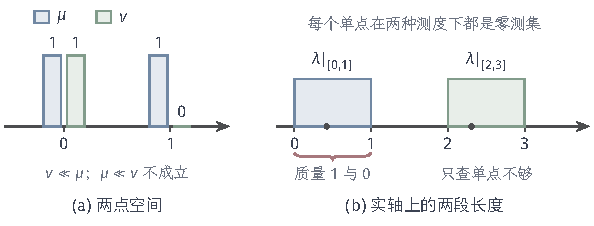
\includegraphics[width=100.669mm]{figures/02-abstract-mathematics/01-metric-and-measure/tikz/c2-absolute-continuity/figure.pdf}
  \caption{绝对连续比较的是零测集。(a)两点空间上$\mu=\delta_0+\delta_1$（蓝）与$\nu=\delta_0$（绿）：$\mu$只把空集看作零测集，所以$\nu\ll\mu$；$\nu$在点$1$的质量为零而$\mu$不为零，所以反向不成立。(b)$\lambda|_{[0,1]}$（蓝）与$\lambda|_{[2,3]}$（绿）在每个单点上都为零，但在$[0,1]$上分别为$1$与$0$，两者互不绝对连续。}
  \label{fig:dens-absolute-continuity}
\end{figure}

\paragraph{与函数的绝对连续}
名称“绝对连续”在第~\ref{chap:integration}章已经用于函数：区间上的函数若在总长度很小的有限个小区间上增量之和也很小，就称它绝对连续。两个概念分别定义，联系要等到第~\ref{sec:dens-cumulative-density}小节才说明：单调函数绝对连续，当且仅当它的增量所产生的测度相对于$\lambda$绝对连续。测度的名称也与“小推出小”有关：若$\nu$有限，则$\nu\ll\mu$等价于对每个$\varepsilon>0$存在$\delta>0$，使$\mu(A)<\delta$推出$\nu(A)<\varepsilon$。本章不使用这一刻画，这里不给出证明。

\subsection{测度的相互奇异}
\label{sec:dens-mutual-singularity}

绝对连续描述的是“参考测度忽略的地方，目标测度也忽略”。与它相对的另一种极端是两个测度各自待在对方忽略的区域里，质量完全不重叠。若$\nu(X\setminus N)=0$，就说$\nu$\emph{集中}在可测集$N$上。

\begin{definition}[相互奇异]
\label{def:dens-mutual-singularity}
设$\mu,\nu$是$(X,\mathcal A)$上的非负测度。若存在$N\in\mathcal A$，使
\[
\mu(N)=0,\qquad\nu(X\setminus N)=0 ,
\]
就称$\mu$与$\nu$\term{相互奇异}（mutually singular），记作$\mu\perp\nu$。
\end{definition}

定义对两个测度是对称的：令$N'=X\setminus N$，则$\nu(N')=0$且$\mu(X\setminus N')=0$，同一关系从$\nu$的角度看就是用补集作分割。直观地说，$X$被一个可测集合分成两块，$\nu$的全部质量在$N$中，$\mu$的全部质量在$X\setminus N$中。在实轴上取$\mu=\lambda|_{[0,1]}$，$\nu=\tfrac12\delta_{1/2}$，$N=\{1/2\}$，则$\mu(N)=0$，$\nu(\mathbb R\setminus N)=0$，所以$\mu\perp\nu$。点$1/2$位于区间内部，相互奇异并不要求两种质量在位置上分开。

两种关系检查的是不同的事。$\nu\ll\mu$问的是$\mu$零测集上有没有$\nu$质量；$\nu\perp\mu$问的是$\nu$能否全部放进一个$\mu$零测集。二者几乎不能同时成立：若$\nu\ll\mu$且$\nu\perp\mu$，取定义中的$N$，则$\mu(N)=0$推出$\nu(N)=0$，又$\nu(X\setminus N)=0$，所以$\nu(X)=0$，$\nu$是零测度。一般的测度两种关系都不满足，例如$\lambda|_{[0,1]}+\delta_2$相对于$\lambda$，第~\ref{sec:dens-decomposition}节将把它拆成满足两种关系的两部分。

\paragraph{集中集合与闭支撑}
在实轴或$\mathbb R^d$上，“相互奇异”很容易被想象成两团质量隔着一段距离。为了说明这种想象不对，先定义Borel测度$\mu$的\term{闭支撑}（support of a measure）：它是这样一些点$x$的集合，$x$的每个开邻域都有正的$\mu$质量。闭支撑的补集是所有$\mu$零测开集之并，因而闭支撑是闭集。$\lambda|_{[0,1]}$的闭支撑是$[0,1]$，$\delta_{1/2}$的闭支撑是$\{1/2\}$，两者相交，测度却相互奇异。

\begin{example}[闭支撑相同而相互奇异]
\label{ex:dens-rationals}
设$(q_n)_{n\geq1}$列举全部有理数，令
\[
\mu=\sum_{n=1}^\infty2^{-n}\delta_{q_n},\qquad\nu=\sum_{n=1}^\infty2^{-n}\delta_{q_n+\sqrt2},
\]
两者都是总质量为$1$的有限测度。$\mu$集中在$\mathbb Q$上，$\nu$集中在$\mathbb Q+\sqrt2$上。这两个集合不相交：若$q=q'+\sqrt2$，则$\sqrt2=q-q'$是有理数，矛盾。取$N=\mathbb Q+\sqrt2$，有$\mu(N)=0$，$\nu(\mathbb R\setminus N)=0$，所以$\mu\perp\nu$。

另一方面，$\mathbb Q$与$\mathbb Q+\sqrt2$都在实轴上稠密，每个非空开区间中两者都有点，所以两个测度在每个非空开区间上都有正质量，闭支撑都是整条实轴。图~\ref{fig:dens-mutually-singular}画出了两组点中的前几个，它们彼此交错。
\end{example}

\begin{figure}[!htbp]
  \centering
  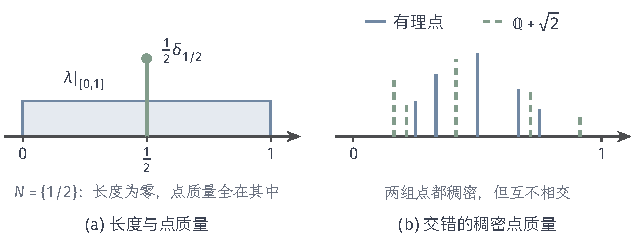
\includegraphics[width=107.668mm]{figures/02-abstract-mathematics/01-metric-and-measure/tikz/c2-mutually-singular/figure.pdf}
  \caption{相互奇异是可测集合上的分离。(a)$\lambda|_{[0,1]}$与$\tfrac12\delta_{1/2}$相互奇异，分离集$N=\{1/2\}$位于区间内部。(b)$\mu=\sum_n2^{-n}\delta_{q_n}$集中在有理点上（蓝色实线），$\nu=\sum_n2^{-n}\delta_{q_n+\sqrt2}$集中在$\mathbb Q+\sqrt2$上（绿色虚线）；图中只画出$[0,1]$内各几个点，线高仅示意权重递减。两组点在每个开区间中都出现，但互不相交，所以$\mu\perp\nu$。}
  \label{fig:dens-mutually-singular}
\end{figure}

这个例子说明，判断相互奇异要找可测的集中集合，而不是看闭支撑是否相交。反方向的蕴含是成立的：若两个闭支撑不相交，取$N$为$\nu$的闭支撑，则$\nu(X\setminus N)=0$：闭支撑的补集中每点都落在某个中心与半径均为有理数、且含于一个$\nu$零测开集的球内，这样的球只有可数个，所以补集是可数个$\nu$零测集之并，而$N$落在$\mu$闭支撑的补集中，$\mu(N)=0$。所以闭支撑不交是相互奇异的充分条件，不是必要条件。顺带一提，上例中的$\mu,\nu$都集中在可数集上，因而都与$\lambda$相互奇异。
